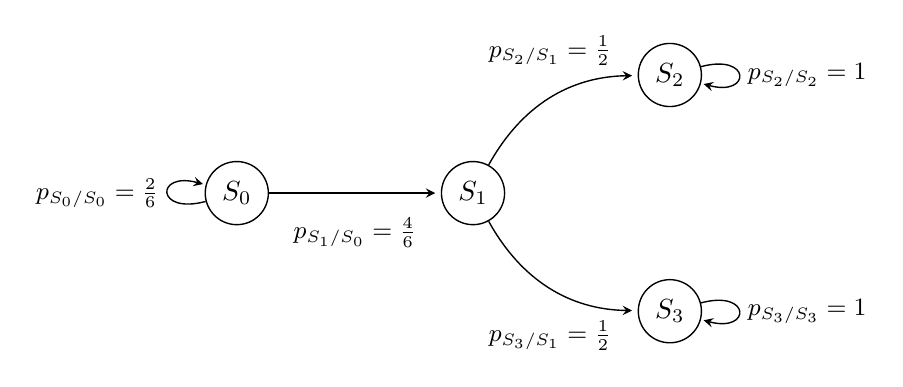
\begin{tikzpicture}[->, >= stealth, shorten >=2pt, line width=0.5pt, node distance=2cm]
  \node[circle, draw] (A) at (0, 1.5) {$S_0$};
  \node[circle, draw] (B) at (3, 1.5) {$S_1$};
  \node[circle, draw] (C) at (5.5, 3) {$S_2$};
  \node[circle, draw] (D) at (5.5, 0) {$S_3$};
  
  \begin{small}
    \path (A) edge [loop left] node [left] {$p_{S_0/S_0} = \frac{2}{6}$} (A);
    \path (A) edge node [below = 0.2cm] {$p_{S_1/S_0} = \frac{4}{6}$} (B);
  
    \path (B) edge [bend left] node [above = 0.3cm] {$p_{S_2/S_1} = \frac{1}{2}$} (C);
    \path (B) edge [bend right] node [below = 0.3cm] {$p_{S_3/S_1} = \frac{1}{2}$} (D);
  
    \path (C) edge [loop right] node {$p_{S_2/S_2} = 1$} (C);
    \path (D) edge [loop right] node {$p_{S_3/S_3} = 1$} (D);
  \end{small}
\end{tikzpicture}
